\documentclass{assignment}
\usepackage[utf8]{inputenc}
\usepackage[T1]{fontenc}
\usepackage{hyperref}

\lstset{
	inputencoding=utf8,
	literate=
	{á}{{\'a}}1
	{é}{{\'e}}1
	{í}{{\'i}}1
	{ó}{{\'o}}1
	{ú}{{\'u}}1
	{Á}{{\'A}}1
	{É}{{\'E}}1
	{Í}{{\'I}}1
	{Ó}{{\'O}}1
	{Ú}{{\'U}}1
	{ñ}{{\~n}}1
	{Ñ}{{\~N}}1
}
\begin{document}
	
	\assignmentTitle{Claudio Iván Esparza Castañeda}{Luis Alberto Balam Guzmán}{./Logo.png}{Maestría en Sistemas Embebidos}{Programación y Procesamiento de Datos}{2A. Práctica de manipulación y organización de datos en Python}
	
	\section*{Objetivo}
	Dentro del estándar de Python se definen múltiples colecciones: listas, tuplas, diccionarios y conjuntos. Las definiciones de cada una, además de sus propiedad y su uso se abordaron en clase, y a través de esta práctica se explora la implementación de la mayoría de ellas.\\
	Combinando los conocimientos usados en la páctica anterior, se combina para tener clases, listas iterables, y un montón de combinaciones en la estructura del proyecto. Dependiendo de las decisiones de diseño se puede ir por un camino u otro para lograr alcanzar los objetivos de requerimientos (de la práctica, en este caso).\\
	Este programa involucra el uso de un menú para el control del flujo. Se cuenta con validaciones para los distintos tipos de datos que se emplean en el programa, y se cuenta con una Clase "Sensor" con métodos para cada etapa opción del menú.
	\section*{Pseudocódigo}
	\lstinputlisting[caption={Datos de sensores}, label={lst:sensores}]{Sensores.psc}
	\section*{Capturas de ejecución}
	\begin{figure}[htbp]
  		\centering
  		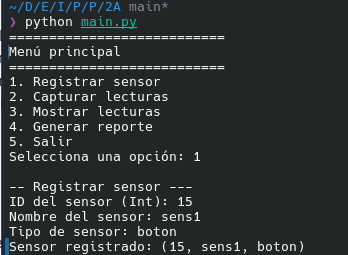
\includegraphics[width=0.5\textwidth]{Figuras/1}
  		\caption{Registro de sensores}
  		\label{fig:1}
	\end{figure}
	\begin{figure}[htbp]
  		\centering
  		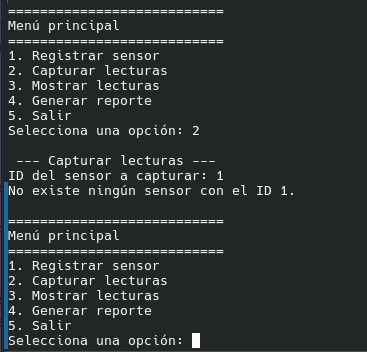
\includegraphics[width=0.5\textwidth]{Figuras/2}
  		\caption{Captura de lecturas. Sensore no válido.}
  		\label{fig:2}
	\end{figure}
	\begin{figure}[htbp]
  		\centering
  		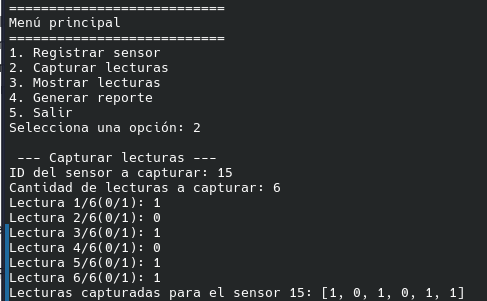
\includegraphics[width=0.5\textwidth]{Figuras/3}
  		\caption{Captura de lecturas. Cantidad de lecturas igual a cero y lectura correcta.}
  		\label{fig:3}
	\end{figure}
	\begin{figure}[htbp]
  		\centering
  		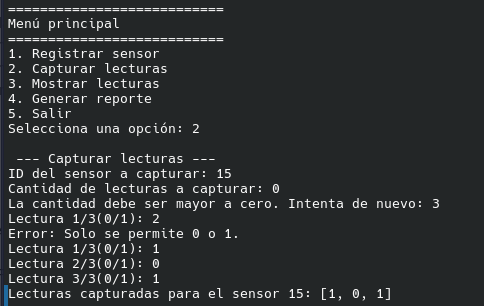
\includegraphics[width=0.5\textwidth]{Figuras/4}
  		\caption{Mostrar lecturas}
  		\label{fig:4}
	\end{figure}
	\begin{figure}[htbp]
  		\centering
  		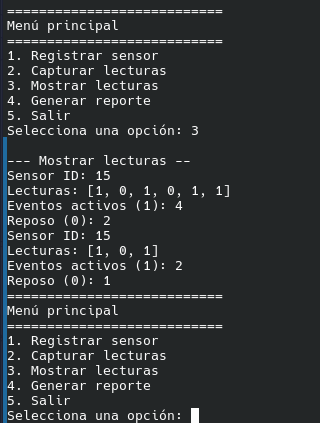
\includegraphics[width=0.5\textwidth]{Figuras/5}
  		\caption{Generar reporte}
  		\label{fig:5}
	\end{figure}
	\section*{Conclusiones}
	Se empleó una estructura basada en la tarea anterior para el menú, y mejorando la función de la validación de los datos para los textos, enteros y binarios. Se creó la clase Sensores y sus diferentes métodos, uno para cada opción. De la misma forma, el constructor de la clase contiene las declaraciones para la lista de tuplas y la lista de lecturas de sensores..
	La carpeta en el repositorio de este proyecto es: \href{https://github.com/clivan/Programacion_y_Procesamiento_de_Datos_Infotec/2A}{Programación y procesamiento de Datos}.	
\end{document}
